\subsubsection{Sistema de autorregulación de humedad}

Para el sistema de autorregulación de humedad, se planteo la idea de mantener húmeda la mezcla a través de un sistema de riego por goteo. 

Este tipo de sistemas se caracteriza por tener una gran eficiencia al momento del riego de huertos e invernaderos cerrados, además de que no desperdician agua. 

Este tipo de riegos se han construido con elementos electrónicos y con un sistema de control ON/OFF.

De esta manera se controla por medio de la generación de un pulso alto con un periodo de tiempo que mantenga encendida la bomba para el riego.

Para el funcionamiento del mismo, será necesario contar con una bomba de agua sumergible, para lo cual, se propuso trabajar con la bomba mostrada en la tabla\ref{tab:bomba}.

\begin{table}[h!]
    \centering
    \caption{Características de la bomba sumergible de agua}
        \begin{tabular}{ |c|c|c|c| } 
            \hline
            \multirow{6}{10em}{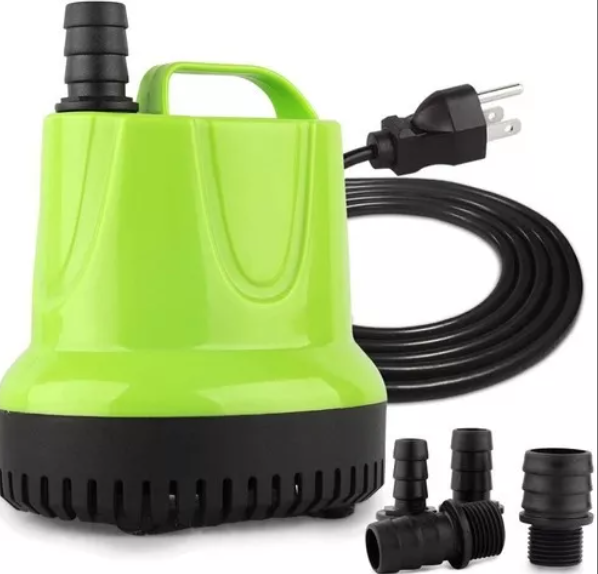
\includegraphics[scale=0.1]{images/Capitulo 4/s5/bomba.png}} & \cellcolor[rgb]{ .851,  .851,  .851}Alimentación & \cellcolor[rgb]{ .851,  .851,  .851} 110-120 V AC a 60 H \\ 
            & Altura de bombeo & 2.5 m \\ 
            & \cellcolor[rgb]{ .851,  .851,  .851}Flujo & \cellcolor[rgb]{ .851,  .851,  .851}2500 \(\frac{L}{H}\) \\ 
            & Potencia &  40 Wats \\
            & \cellcolor[rgb]{ .851,  .851,  .851}Dimensiones & \cellcolor[rgb]{ .851,  .851,  .851}13 x 11 x 9 cm \\
             \hline
        \end{tabular}
    \label{tab:bomba}%
\end{table}

Esta bomba esta conectada a un sistema de tuberías que se fabricaron con tubos de PVC, para llevar el liquido al interior del contenedor. 

Este sistema de tuberías tiene un diámetro 1 pulgada y eleva el liquido que esta en un contenedor del piso a un metro de altura. Al interior del contenedor se encuentra un tubo de PVC con una perforación cada 10 cm, para permitir el riego de la mezcla. 
